\chapter{Organizzazione del progetto}	
		
		\section{Organizzazione strutturale}
		\label{sec:struc}
		
		La struttura organizzativa del progetto risulta difficile da stabilire in questa fase preliminare. In fasi più avanzate, i team member potranno essere suddivisi in team dedicati ad attività specifiche (Es. team di implementazione, team di testing).
		
		\begin{figure}[ht]
		\centering
		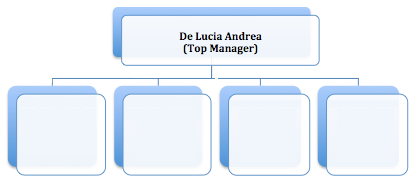
\includegraphics[width=\textwidth]{img/organizzazione.png}
		\caption{Struttura organizzativa}\label{fig:1}
		\end{figure}
		
		\newcolumntype{C}[1]{>{\centering}p{#1}}
		\begin{table}[ht]
		\centering
			\begin{tabular}{|C{4cm}|C{4cm}|C{4cm}|}
				\hline
				\textbf{Nome componente} & \textbf{Ruolo} & \textbf{Responsabilità}\tabularnewline
				\hline
				Matteo Merola & Team member & Sviluppo deliverables: DL1, DL2, DL3, DL6, DL8, DL9, DL12\tabularnewline
				\hline
				Simone Scalabrino & Team member & Sviluppo deliverables: DL1, DL2, DL4, DL5, DL7, DL10, DL11, DL12\tabularnewline
				\hline
				Giovanni Grano & Team member & Sviluppo deliverables: DL1, DL2, DL3, DL6, DL8, DL9, DL12\tabularnewline
				\hline
				Carlo Branca & Team member & Sviluppo deliverables: DL1, DL2, DL4, DL5, DL7, DL10, DL11, DL12\tabularnewline
				\hline
			\end{tabular}
		\caption{Ruoli e responsabilità}
		\label{proj_org:ruoli}
		\end {table}